\chapter{Logistična regresija}
\label{ch:logistic-regression}

V zgornjem delotoku smo uporabili logistično regresijo, priljubljeno metodo strojnega učenja. Pogosto se uporablja v rudarjenju besedil zaradi hitrosti in napovedne točnosti. Kako pa deluje?

\begin{figure}
    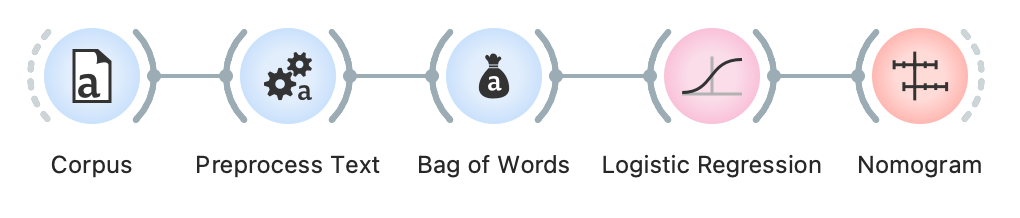
\includegraphics[width=\textwidth]{logisticna-workflow.png}
    \caption{ }
\end{figure}

Pri postopku besede glasujejo. Na primer, beseda ‘fox’ v besedilu glasuje, da je pravljica živalskega tipa. Enako glasujejo mačke, ptiči in volkovi, ampak manj močno (črte v vizualizaciji so krajše). Lisica je očitno najboljši namig, da je pravljica živalska.\marginnote{Vizualizacija se imenuje nomogram in prikaže točke (glasove) za najboljših 6 spremenljivk za ciljno vrednost, ki je izbrana levo zgoraj}

Beseda ``little'' glasuje obratno. Ravno tako beseda ``came'' (opazite, kako imajo te besede ničlo na desni strani črte?). Vsaka beseda prispeva h končni oceni. Če v pravljici ni besede ``majhen'', potem živalskim pravljicam dodeli 5 točk. In če je v besedilu 29 lisic, potem model dodeli 3 točke za živalske pravljice. 

Jasno je dejanska metoda nekoliko bolj zapletena, saj poskuša najti pravilno ravnotežje med utežmi glasov in mejami odločitve. Ampak to vsebuje kot volk strašno linearno algebro, tako da se raje ne bomo podali na to pot.

\begin{figure}
    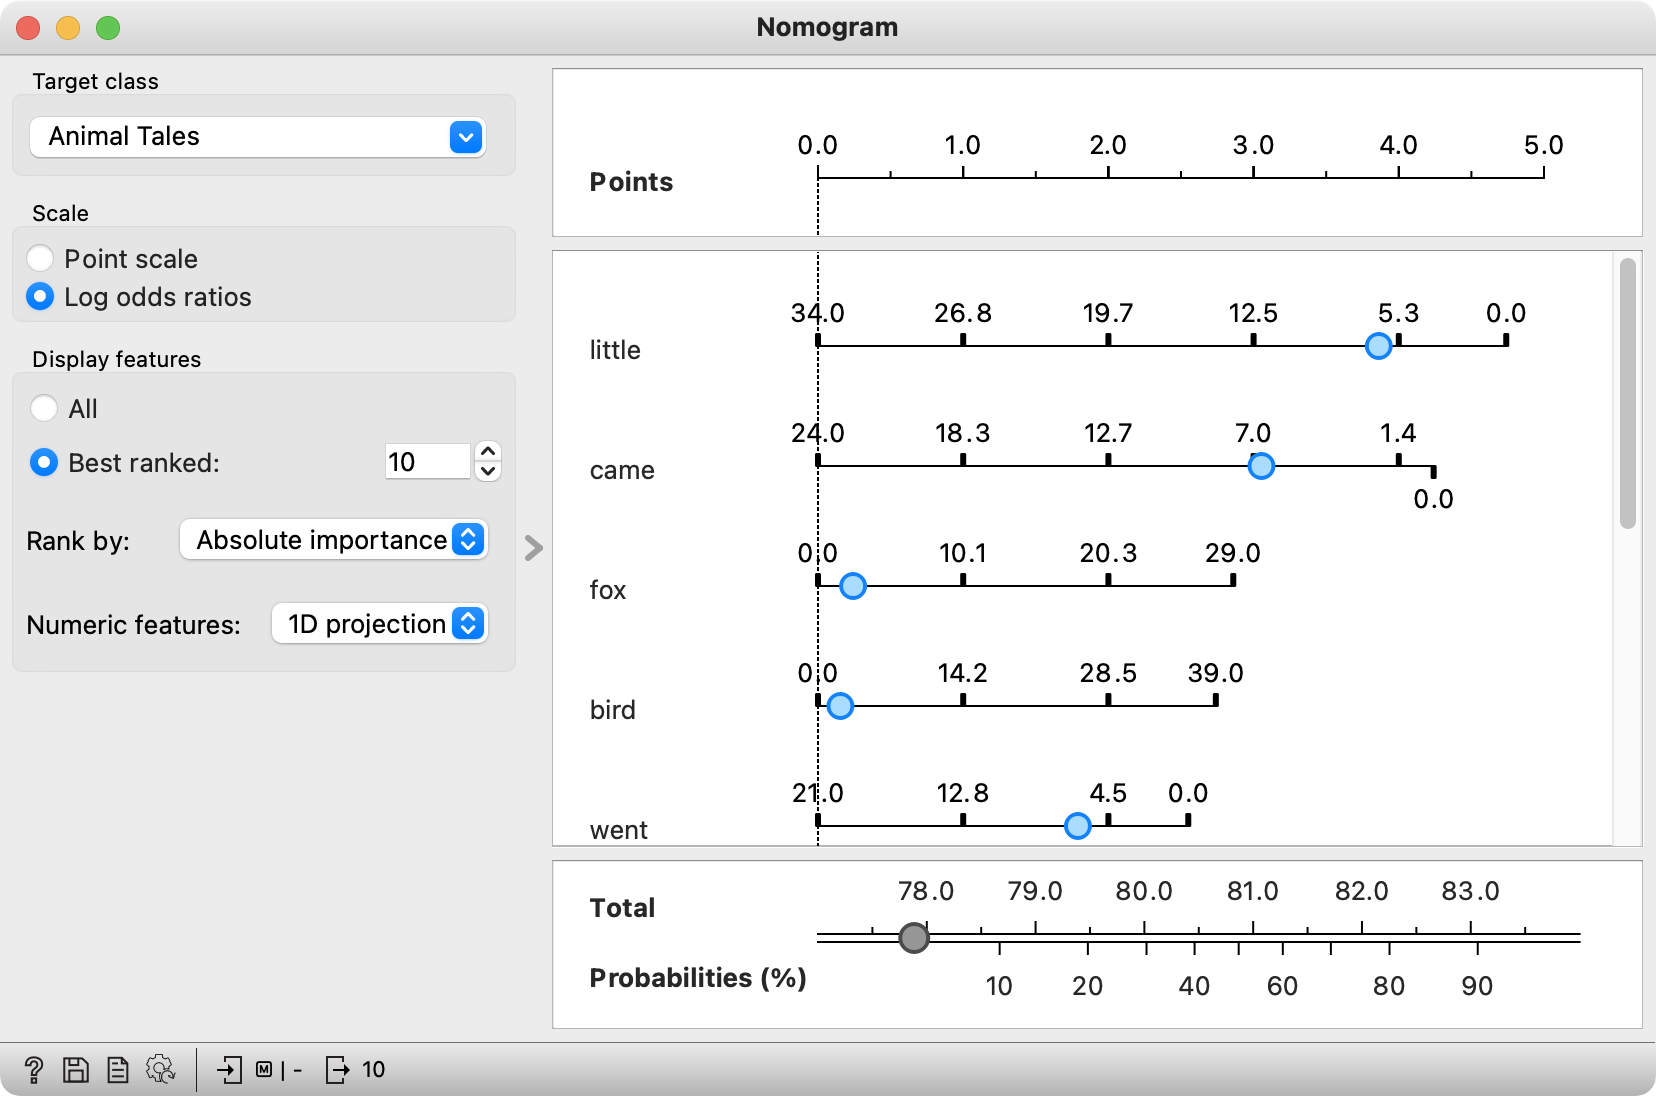
\includegraphics[width=\textwidth]{nomogram.png}
    \caption{V gradniku Nomogram lahko interaktivno opazujete odločitve modela. Povlecite modre točke levo ali desno tako, da bo končna vsota točk (Total) kar največja.}
\end{figure}
